\part{Korespondence svazků}

Kámen vložený do měřicí soustavy vytvoří na stínítku specifický obrazec. Pokud vytvoříme vhodný matematický model této situace a aplikujeme na něj optické zákony, dostaneme stejný obrazec. 

Úloha optimalizace náklonu faset spočívá v nalezení korespondujících svazků. Korespondence je uspořádaná dvojice měřeného a referenčního svazku. Korespondující svazky mají společnou posloupnost dopadových faset. 

\section{Složitost úlohy}
	Korespondence nelze nalézt všechny najednou. Ve snímku \ref{fig: kores_faze_0} jsou zobrazeny vzdálenosti korespondujících svazků po optimalizaci náklonu a rotace kamene. Vzdálenost většiny korespondujících svazků je příliš vysoká na to, abychom mohli korespondence nalézt. Situace je navíc komplikována tím, že řada referenčních svazků, kterým v odraze odpovídá měřený svazek neexistuje. Ve fázi optimalizace na obrázku \ref{fig: kores_faze_0} neexistuje \SI{36}{\percent} referenčních svazků, k nimž později přiřadíme korespondující měřený svazek. 
	
	  V prvním kroku lze nalézt korespondence pouze pro vybrané třídy svazků. Jedná se o třídy \textbf{1A}, \textbf{3A} a ne vždy detekované třídy \textbf{3B} a \textbf{5D} viz obr. \ref{fig:wedge_example_image}. 
	
	Čekali bychom, že pokud optimalizujeme náklon faset s korespondencemi svazků, které lze určit v počátku, budou obrazy ostatních korespondujících svazků téměř totožné. Na obr. \ref{fig: kores_faze_1} ovšem vidíme, že ani v tomto případě nelze určit všechny korespondence. Vzdálenosti obrazů korespondujících svazků stále znatelné. Zvláště pak máme problém nalézt korespondence v oblastech s vysokou hustotou svazků. Je zřejmé, že korespondence budeme muset nacházet ve více krocích a postupně parametry faset přibližovat ke konečnému výsledku náklonu. 

Indikátorem, zda jsme nastavili správně parametry faset kamene, je vzdálenost měřených a referenčních svazků. Po optimalizaci náklonu faset podle korespondujících svazků (obr. \ref{fig: kores_faze_2}) vidíme, že směry korespondujících svazků v mnoha případech nesouhlasí. Navíc můžeme pozorovat měřené svazky, ke kterým neexistuje vhodný referenční svazek a naopak vidíme také volné referenční svazky. Na tyto nepřesnosti má vliv zakřivení faset, neurčitost vzdálenosti faset, nepřesná kalibrace, detekce atd.  

 
 \begin{figure}[htbp]
    \centering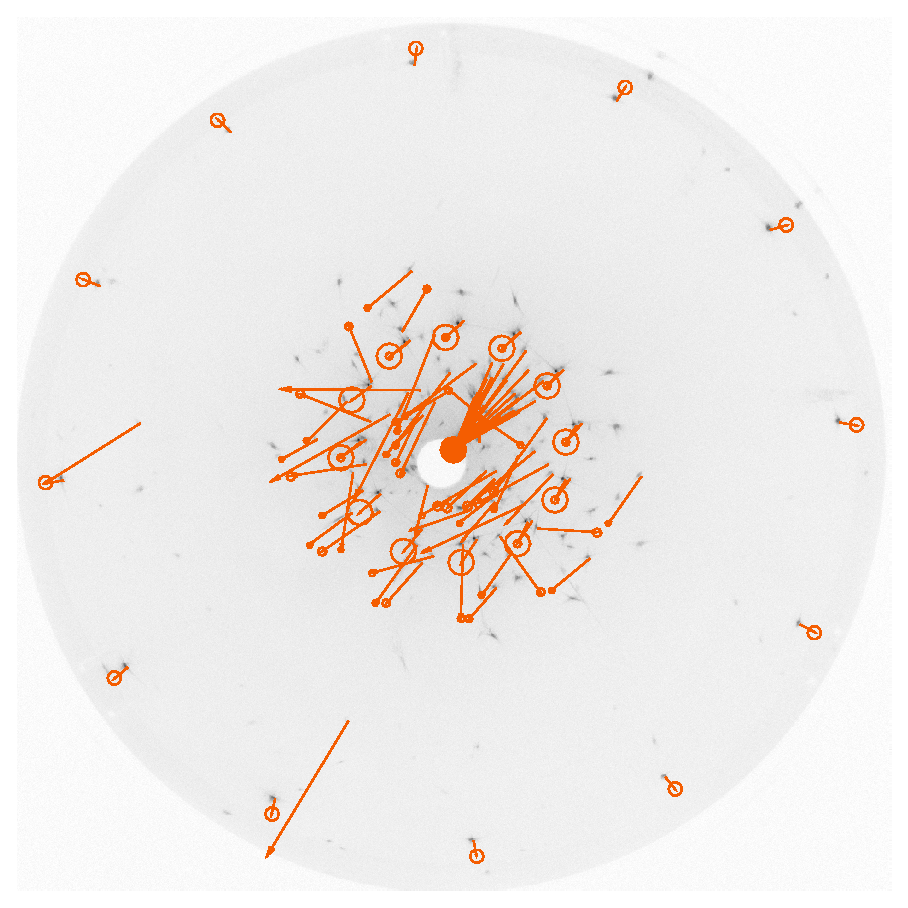
\includegraphics[width=\textwidth]{kores_faze_1.eps}
    \caption[Vzdálenost korespondujících svazků - fáze 0.]{Vzdálenost korespondujících svazků po optimalizaci náklonu a rotace kamene \textit{viva12}. Kružnice znázorňují referenční svazky. Čím vyšší je zářivý tok svazku, tím vyšší je poloměr kružnice. Vektory směřují od obrazu měřeného svazku k obrazu korespondujícího referenčního svazku. Modrou barvou jsou zobrazeny referenční svazky, pro které nebyl nalezen korespondující měřený svazek.}
 \label{fig: kores_faze_0}
 \end{figure}

 
 \begin{figure}[htbp]
    \centering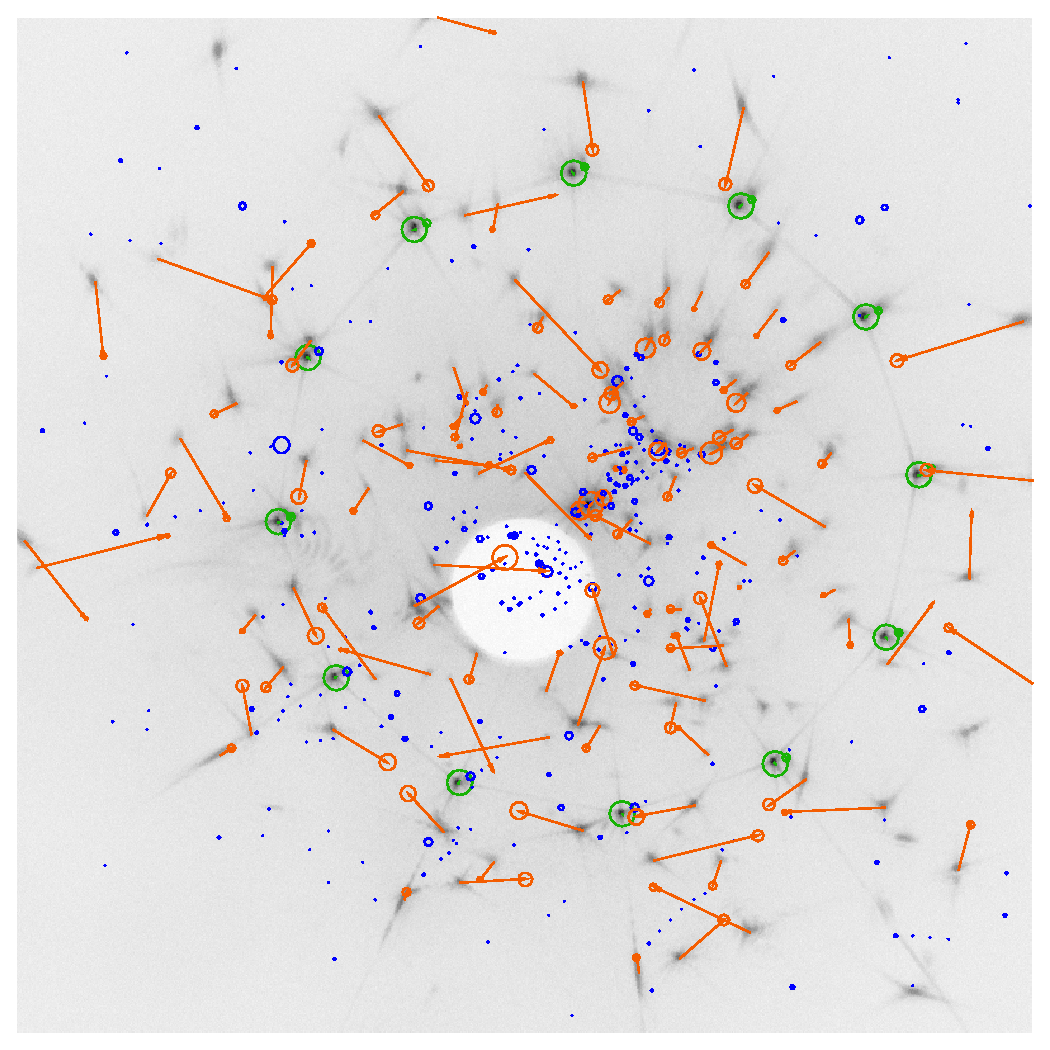
\includegraphics[width=\textwidth]{kores_faze_3.eps}
    \caption[Vzdálenost korespondujících svazků - fáze 1.]{Vzdálenost korespondujících svazků po optimalizaci náklonu faset podle korespondencí, které lze spolehlivě nalézt. Kružnice znázorňují referenční svazky. Čím vyšší je zářivý tok svazku, tím vyšší je poloměr kružnice. Vektory směřují od obrazu měřeného svazku k obrazu korespondujícího referenčního svazku. Zelenou barvou jsou zobrazeny korespondence použité při optimalizaci parametrů kamene. Modrou barvou jsou zobrazeny referenční svazky, pro které nebyl nalezen korespondující měřený svazek. Detail na střední část snímku.}
 \label{fig: kores_faze_1}
 \end{figure}
 
  \begin{figure}[htbp]
    \centering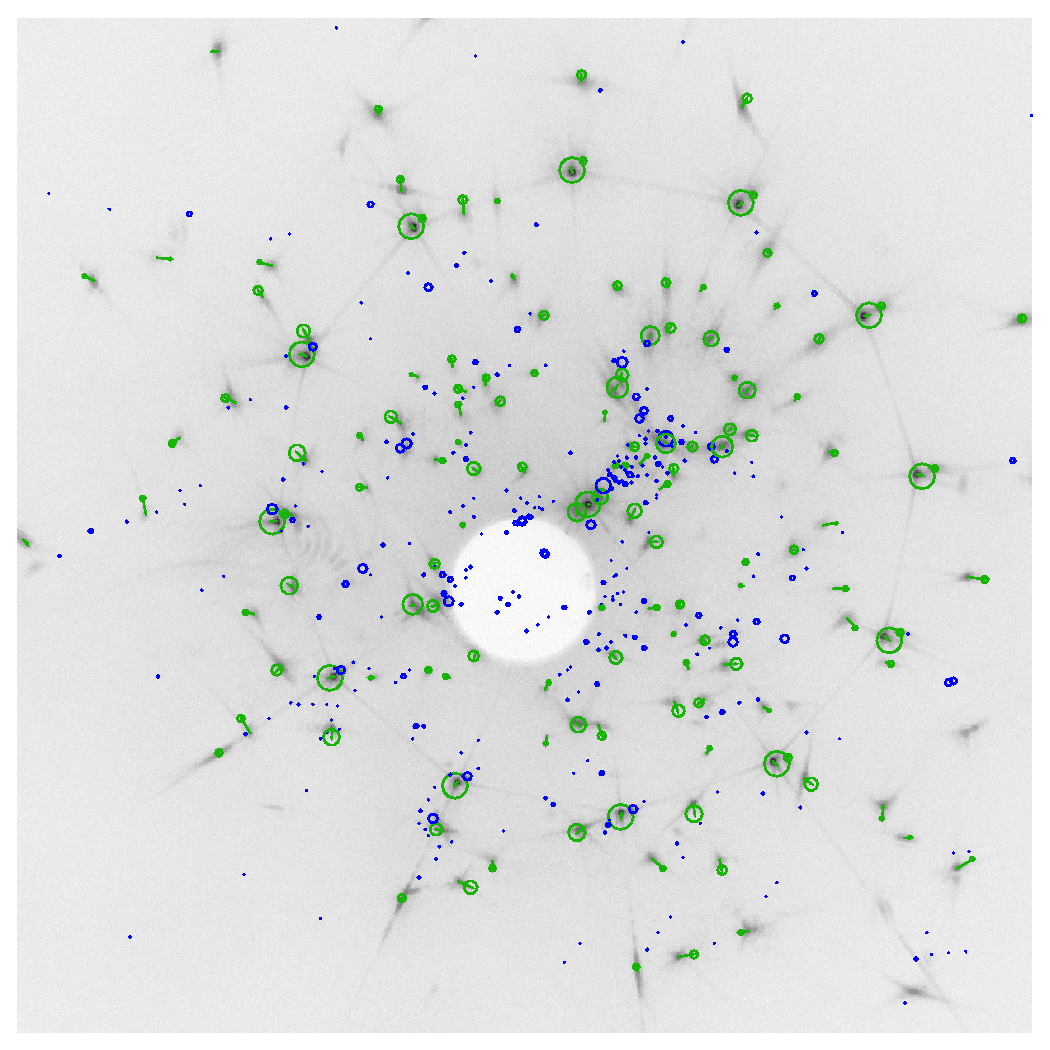
\includegraphics[width=\textwidth]{kores_faze_4.eps}
    \caption[Vzdálenost korespondujících svazků - konečná fáze.]{Vzdálenost korespondujících svazků po optimalizaci náklonu faset podle všech korespondujících svazků. Kružnice znázorňují referenční svazky. Čím vyšší je zářivý tok svazku, tím vyšší je poloměr kružnice. Vektory směřují od obrazu měřeného svazku k obrazu korespondujícího referenčního svazku. Zelenou barvou jsou zobrazeny korespondence použité při optimalizaci parametrů kamene. Modrou barvou jsou zobrazeny referenční svazky, pro které nebyl nalezen měřený svazek. Detail na střední část snímku. }
 \label{fig: kores_faze_2}
 \end{figure}
 
 \clearpage